\documentclass{article}

%Page format
\usepackage[table]{xcolor}
\usepackage{pdfpages}
\usepackage{fancyhdr}
\usepackage[margin=1in]{geometry}
\usepackage{tabularx}
%Math packages and custom commands
\usepackage{algpseudocode}
\usepackage{amsthm}
\usepackage{framed}
\usepackage[margin=1in]{geometry}
\usepackage{hyperref}
\usepackage{tikz}
\usepackage[utf8]{inputenc}
\definecolor{Gray}{gray}{0.9}
\usepackage{wrapfig}
\usepackage[margin=1in]{geometry}
\usepackage{mathtools,amsthm}
\usepackage{enumitem,amssymb}
\newtheoremstyle{case}{}{}{}{}{}{:}{ }{}
\theoremstyle{case}
\newtheorem{case}{Case}
\DeclareMathOperator{\R}{\mathbb{R}}
\DeclareMathOperator{\E}{\mathbb{E}}
\DeclareMathOperator{\Var}{\text{Var}}
\DeclareMathOperator{\Cov}{\text{Cov}}
\newcommand{\bvec}[1]{\mathbf{#1}}
\renewcommand{\P}{\mathbb{P}}
\newcommand{\norm}[2][2]{\| #2\|_{#1}}

\definecolor{shadecolor}{gray}{0.9}

\theoremstyle{definition}
\newtheorem*{answer}{Answer}
\newcommand{\note}[1]{\medskip \noindent{\textbf{NOTE:} #1}}
\newcommand{\hint}[1]{\medskip \noindent{\textit{HINT:} #1}}
\newcommand{\recall}[1]{\medskip{[\textbf{RECALL:} #1]}}
\newcommand{\motivation}[1]{\medskip \noindent{\textbf{MOTIVATION:} #1}}
\newcommand{\expect}[1]{\medskip \noindent{\fbox{\parbox{0.95 \textwidth}{\medskip \textbf{What we expect:} #1}}}}
\newcommand{\solution}{
    {
        \begin{shaded}
            \textbf{Your Solution:}
        \end{shaded}
        \pagebreak
    }
}
\newcommand{\mysolution}[1]{\medskip{\begin{shaded}\textbf{Your Solution:}\ #1 \end{shaded}}}
\newlist{todolist}{itemize}{2}
\setlist[todolist]{label=$\square$}
\usepackage{pifont}
% use below to modify the size of equations
% usage is as follows: {fontsize}{math text size}{subscript size}{subsubscript size}
% if you wish to change the math font size, modify {math text size}{subscript size}{subsubscript size} for your chosen global font size {fontsize} which is declared at the beginning of the document
\DeclareMathSizes{10}{13}{13}{13}
\DeclareMathSizes{14}{17}{17}{17}
\DeclareMathSizes{12}{15}{15}{15}
\newcommand{\cmark}{\ding{51}}%
\newcommand{\xmark}{\ding{55}}%
\newcommand{\done}{\rlap{$\square$}{\raisebox{2pt}{\large\hspace{1pt}\cmark}}%
\hspace{-2.5pt}}
\newcommand{\wontfix}{\rlap{$\square$}{\large\hspace{1pt}\xmark}}
\graphicspath{ {./images/} }

\title{\textbf{CS221 Autumn 2021: Artificial Intelligence:\\ Principles and Techniques} \\Homework 7: Car Tracking}
\date{}

\chead{Car}
\rhead{\today}
\lfoot{}
\cfoot{CS221: Artificial Intelligence: Principles and Techniques --- Autumn 2021}
\rfoot{\thepage}
\renewcommand{\headrulewidth}{0.4pt}
\renewcommand{\footrulewidth}{0.4pt}
\pagestyle{fancy}
\setlength{\parindent}{0pt}


\begin{document}
	
\maketitle


\begin{center}
\begin{tabular}{rl}
SUNet ID: & [your SUNet ID] \\
Name: & [your first and last name] \\
Collaborators: & [list all the people you worked with]
\end{tabular}
\end{center}
\newcolumntype{g}{>{\columncolor{Gray}}c}
\textit{By turning in this assignment, I agree by the Stanford honor code and declare
that all of this is my own work.} \\
% uncomment one of the below lines to make the text larger
\fontsize{12pt}{16pt}\selectfont

\textbf{Collaborators: [insert names here]}

\textit{By turning in this assignment, I agree by the Stanford honor code and declare that all of this is my own work.} \\
%%%%%%%%%%%%%%%%%%%%%%%%%%%%%%%%%%%%%%%%%%%%%%%%%%%%%%%%%%%%%%%%%%%%%%%%%%%%%%%%
\section*{Problem 4 : Which car is it?}


So far, we have assumed that we have a distinct noisy distance reading for each car, but in
reality, our microphone would just pick up an undistinguished set of these signals, and we
wouldn't know which distance reading corresponds to which car.
First, let's extend the notation from before: let $C_{ti} \in \mathbb R^2$ be the location
of the $i$-th car at the time step $t$, for $i = 1, \dots, K$ and $t = 1, \dots, T$.
Recall that all the cars move independently according to the transition dynamics as before.\\


Let $D_{ti} \in \mathbb R$ be the noisy distance measurement of the $i$-th car at time step $t$,
which is now not directly observed.
Instead, we observe the unordered set of distances
$\{ D_{t1}, \dots, D_{tK} \}$ as a collective and so cannot attribute any individual measurement in this set to a specific car.  (For simplicity, we'll assume that all distances are distinct values.)
In other words, you can think of this scenario as the same as observing the list $\mathbf{E_t} = [E_{t1}, \dots, E_{tK}]$
which is a uniformly random permutation of the (noisy) correctly ordered distances $\mathbf{D_t} = [D_{t1}, \dots, D_{tK}]$ where index $i$ represents the noisy distance to car $i$ at time $t$.\\

For example, suppose $K=2$ and $T = 2$.
Before, we might have gotten distance readings of $8$ and $4$ for the first car and
$5$ and $7$ for the second car at time steps $1$ and $2$, respectively.
Now, our sensor readings would be permutations of $\{8, 5\}$ (at time step $1$) and $\{4, 7\}$ (at time step $2$).
Thus, even if we knew the second car was distance $5$ away at time $t = 1$,
we wouldn't know if it moved further away (to distance $7$) or closer (to distance $4$) at time $t = 2$.\\

Here is a diagram that shows the flow of information corresponding to the above situation for the case where $K = 2$ and only showing two timesteps, $t$ and $t+1$. Note that because the observed distances $\mathbf{E_t}$ are a permutation of the true distances $\mathbf{D_t}$, each $E_{ti}$ depends on all of the $D_{ti}$. Also note that the above diagram is not a Bayes net as $E_{t1}$ and $E_{t2}$ are not conditionally independent given $D_{t1}$ and $D_{t2}$ (however, $D_{t1}$ and $D_{t2}$ are conditionally independent given $C_{t1}$ and $C_{t2}$)



\begin{center}
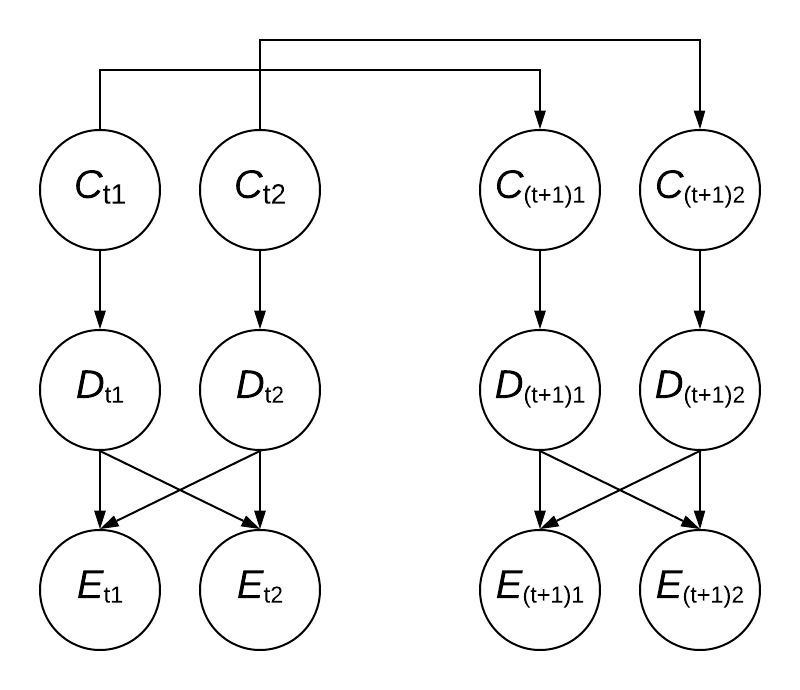
\includegraphics[width=60mm]{images/Q4_diag.jpeg}
\end{center}
%%%%%%%%%%%%%%%%%%%%%%%%%%%%%%%%%%%%%%%%%%%%%%%%%%%  a
	\begin{enumerate}
	\item[a.] [5 points] Suppose we have $K=2$ cars and one time step $T=1$.
    Write an expression for the conditional probability
    $p(C_{11} = c_{11}, C_{12} = c_{12} \mid \mathbf{E_1} = \mathbf{e_1})$
    as a function of the PDF of a Gaussian $ p_{\mathcal N}(v; \mu, \sigma^2)$
    and the prior probability $p(c_{11})$ and $p(c_{12})$ over car locations.
    Your final answer should not contain variables $D_{11}$, $D_{12}$.\\
    
    Remember that $p_{\mathcal N}(v; \mu, \sigma^2)$ is the probability of a random
    variable, $v$, in a Gaussian distribution with mean $\mu$ and standard deviation $\sigma$.\\
	
	\hint{for $K=1$, the answer would be:
	
	$$p(C_{11} = c_{11} \mid \mathbf{E_1} = \mathbf{e_1}) \propto p(c_{11}) p_{\mathcal N}(e_{11}; \|a_1 - c_{11}\|_2, \sigma^2).$$

where $a_t$ is the position of your car (that you are controlling) at time $t$. Remember that $C_{ti}$ is the position of the $i$th observed car at time $t$. To better inform your use of Bayes' rule, you may find it useful to draw the Bayesian network and think about the distribution of $\mathbf{E_t}$ given $D_{t1}, \dots, D_{tK}$.\\}

\hint{Note that the observed variable(s) are the shuffled/randomized distances $\mathbf{E_t}  = [E_{t1}, E_{t2}, ..., E_{tK}]$.
        These are a random permutation of the unobserved noisy distances $\mathbf{D_t} = [D_{t1}, D_{t2}, ..., D_{tK}]$, where $D_{t1}$ is the distance of car $1$ at timestep $t$.
        Note that $E_{t1}$ is the emission from one of the cars at timestep $t$, but we aren't sure which one (it is NOT necessarily car 1, it could be any of the cars).
        On the other hand, $D_{t1}$ is the measured distance of car 1 (we know with certainty that it comes from car 1), the only issue is that we don't observe it directly.
} %TODO

\hint{To reduce notation, you may write, for example, $p(c_{11}\mid e_{11})$ instead of $p(C_{11}=c_{11} \mid E_{11}=e_{11})$.}

\expect{A mathematical expression, with the steps you took to derive that expression, relating (can be proportionality) $p(C_{11} = c_{11}, C_{12} = c_{12} | \mathbf{E_1} = \mathbf{e_1})$ with the PDF of a Gaussian and the priors $p(c_{11})$ and $p(c_{12})$ over car locations.}


\mysolution{

}
    

%%%%%%%%%%%%%%%%%%%%%%%%%%%%%%%%%%%%%%%%%%%%%%%%%%%% b
\newpage
	\item[b.] [4 points] Assuming the prior $p(c_{1i})$ of where the cars start out is the same for all $i$ (i.e. for all K cars),
    show that the number of assignments for all $K$ cars $(c_{11}, \dots, c_{1K})$
    that obtain the maximum value of
    $p(C_{11} = c_{11}, \dots, C_{1K} = c_{1K} \mid \mathbf{E_1} = \mathbf{e_1})$ is at least $K!$ (K factorial).
    You can also assume that the car locations that maximize the probability above
    are unique ($C_{1i} \neq c_{1j}$ for all $i \neq j$).

\hint{The priors $p(c_{1i})$ are a probability distribution over the possible starting positions ($t=1$) of each car $i$. Note that even if the car positions share the same prior, it doesn't necessarily mean they have the exact same start positions $c_{1i}$ because the start positions are sampled from the prior distribution, which can yield different values each time it is sampled from. However, you should think about what the priors all being the same means intuitively in terms of how we can associate observations with cars.}
      
\note{Note: you don't need to produce a complicated proof for this question. It is acceptable to provide a clear explanation based on your intuitive understanding of the scenario.}

\expect{Either a short mathematical argument or concise explanation for why the statement defined in the problem is true.}

\mysolution{

}
%%%%%%%%%%%%%%%%%%%%%%%%%%%%%%%%%%%%%%%%%%%%%%%%%%% c

\item[c.] [2 points, extra credit] For general $K$, what is the treewidth corresponding to the posterior probability over all $K$ car locations at all $T$ time steps conditioned on all the sensor readings:

$$p(C_{11} = c_{11}, \dots, C_{tk} = c_{tk}, \dots, C_{TK} = c_{TK} \mid \mathbf{E_1} = \mathbf{e_1}, \dots, \mathbf{E_T} = \mathbf{e_T})$$

Briefly justify your answer.For reference, the treewidth of a factor graph is defined as the maximum arity (number of variables that a factor depends on) of any factor created by variable elimination under the best variable elimination ordering. You can find further information, along with an example, that may be relevant to this problem \href{https://stanford.edu/~shervine/teaching/cs-221/cheatsheet-variables-models}{here}.

\expect{The treewidth as a function of $K$ and a justification for why the treewidth is represented by that function.}

\begin{figure}[h]
\mysolution{

}
\end{figure}
%%%%%%%%%%%%%%%%%%%%%%%%%%%%%%%%%%%%%%%%%%%%%%%%%%% d
\newpage

\item[d.]  [4 points, extra credit]  Now suppose you change your sensors so that at each time step $t$, they return the list of exact positions of the $K$ cars, but the list of positions is shifted by a random number of indices (with wrap around). For example, if the true car positions at time step $1$ are $c_{11} = (1, 1) , c_{12} = (3, 1), c_{13} = (8, 1), c_{14} = (5, 2)$, then $\mathbf{e_1}$ would be $[(1, 1), (3, 1), (8, 1), (5, 2)]$, $[(3, 1), (8, 1), (5, 2), (1, 1)]$, $[(8, 1), (5, 2), (1, 1), (3, 1)]$, or $[(5, 2), (1, 1), (3, 1), (8, 1)]$, each with probability $1/4$. Describe an efficient algorithm for computing $p(c_{ti} \mid \mathbf{e_1}, \dots, \mathbf{e_T})$ for any time step $t$ and car $i$.  Your algorithm should not be exponential in $K$ or $T$.

\expect{A description of the factor graph/Bayesian net used to model the problem, including any relevant variables and conditional probabilities. Also, a description of how you would use the factor graph to compute the provided probability. Note that you should try to simplify your expression for the probability as much as possible given the information provided.}


\mysolution{

}

%%%%%%%%%%%%%%%%%%%%%%%%%%%%%%%%%%%%%%%%%%%%%%%%%%%%%%%%%%%%%%%%%%%%%%%%%%%%%%%%
\section*{Problem 5 : Ethics in Advanced Technologies}

\begin{enumerate}

\item[a.] [4 points]
You are in charge of public policy for an autonomous vehicle company headquartered in California. 
Your engineering team is making progress in designing a fully automated vehicle and would like to test it on real
roadways. California would require that you apply for autonomous vehicle testing permits and meet regulatory
standards designed to protect the safety of other motorists and pedestrians. Given these regulations,
testing your vehicles in California secretly without a permit would be illegal.
The Governor of Arizona has reached out to offer your company testing in the state without restrictions. 
Doing so would allow you to test more quickly and without making any changes to your vehicles. On the other hand,
testing in Arizona could be considered “ethics dumping,” namely “doing research deemed unethical in a scientist’s
home country in a country or region with laxer ethical rules” and regulations. \\

Would testing in Arizona be “ethics dumping”? Be sure to explain why you think it is  or isn’t. Given your answer to this question and other factors you consider to be relevant, should you perform your tests in Arizona or comply with Californian standards? Justify your answer with a reason as to why.\\

\expect{
    In 3-6 sentences, we expect:
    \begin{enumerate}
        \item a yes or no answer to the ethics dumping question
        \item an explanation of why it is or isn’t ethics dumping given the definition above
        \item a yes or no answer to whether the tests should be done in Arizona or California
        \item an explanation that justifies why the tests should be done in Arizona or California
    \end{enumerate}
}

\mysolution{

}


\item[b.] [3 points] Dual-use technologies are technologies that serve two purposes, typically a military and a civilian purpose. Researchers developing dual-use technologies face a moral dilemma: though they may intend to improve only the peaceful use of the technology, any improvements they make aid others who use the technology in war or in non-state attacks or killings. Tracking of the kind developed in this assignment can be used in self-driving cars or in autonomous weapons systems, such as lethal drones that track people to kill them.\\

Imagine a researcher who develops a dual-use technology despite knowing about the lethal secondary use of the technology and despite the researcher considering this secondary use unethical. Would the researcher be partially morally responsible for  improvements to the lethal use of the technology that result from their discoveries?  If not, give one reason why not. If so, explain why they are partially responsible and explain what action(s) the researcher should take to address this (choosing another line of research, building a safeguard, or other)?

\expect{
    In 3-6 sentences, we expect:
    \begin{enumerate}
        \item answers yes or no to whether the researcher would be partially morally responsible
        \item provides a reason why they would or would not be partially morally responsible
        \item if yes, describes an action they should take
    \end{enumerate}
}

\mysolution{

}

\end{enumerate}


\end{enumerate}

\end{document}